% Figure captions for coordinate-field-generator paper

\begin{figure*}[!htbp]
    \centering
    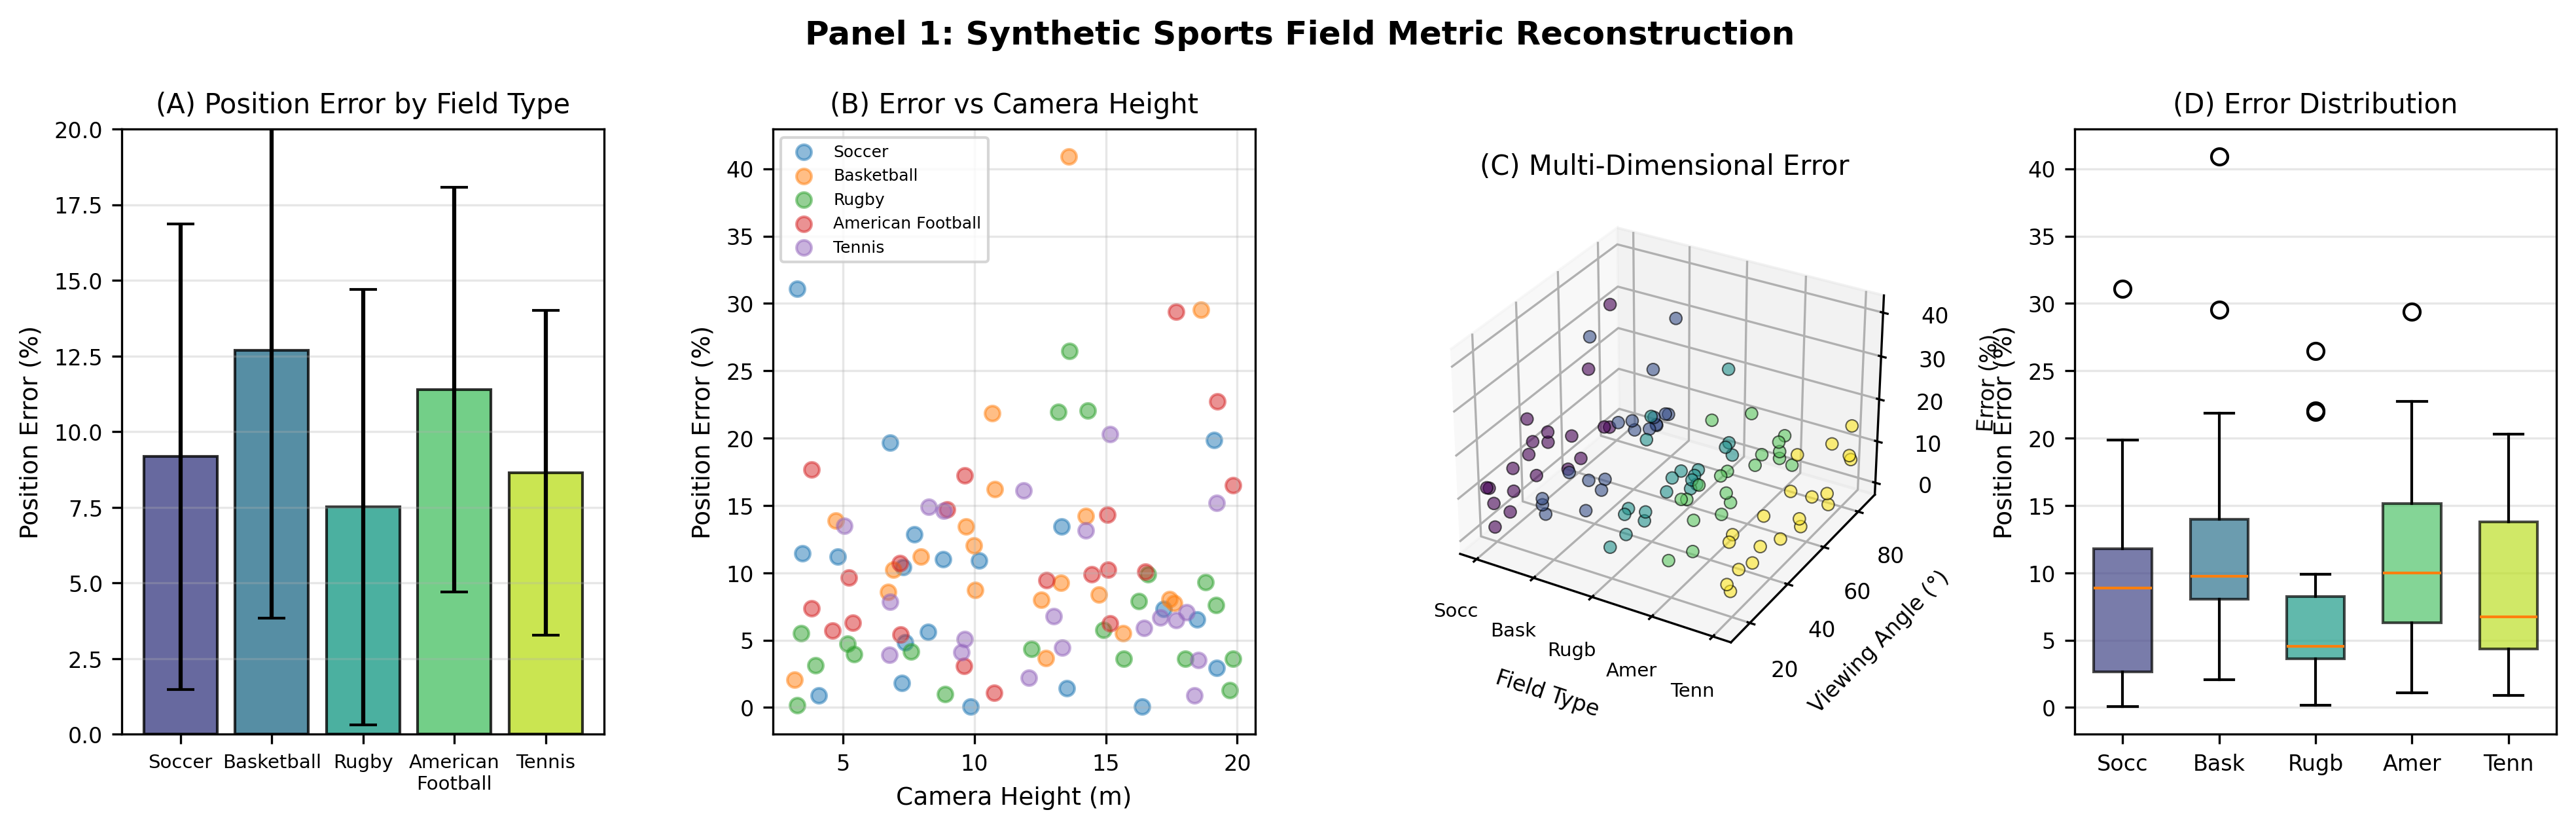
\includegraphics[width=\textwidth]{figures/panel_1_synthetic_fields.png}
    \caption{\textbf{Synthetic sports field metric reconstruction shows mean position errors of 7.5--13\% across five field types, with errors increasing under extreme viewing angles and decreasing with moderate camera heights (20 viewpoints per field type; 5 field types tested: soccer, basketball, rugby, American football, tennis; field diagonal 68--120 m; Theorem~\ref{thm:spectral_geom}).}
    (\textbf{A})~Bar chart of mean position error (percent) for each field type with error bars ($\pm 1$ std dev). Errors range from $7.5\%$ (rugby) to $12.7\%$ (basketball), reflecting different field aspect ratios and characteristic landmark scales. Standard deviations of 5--9\% show substantial trial-to-trial variability.
    (\textbf{B})~Scatter of position error versus camera height above field. Error shows weak correlation with height (range 3--20 m); optimal reconstruction occurs at mid-heights (8--12 m) where perspective foreshortening is moderate. Very high cameras ($>18$ m) show elevated error as viewing angle approaches near-parallel to field plane.
    (\textbf{C})~Three-dimensional scatter of field type (x-axis, indexed 0--4), viewing angle (y-axis, 15--85°), and position error (z-axis, 0--25\%). Point cloud reveals clustering by field type, with tennis showing consistently higher errors across viewing angles. Vertical spread at each field index reflects angle-dependent variability; angle gradient across x reveals interaction between field geometry and perspective.
    (\textbf{D})~Boxplot of error distribution per field type showing median (white line), interquartile range (box), and outliers (red +). All distributions are right-skewed with outliers up to $\approx 20\%$, indicating occasional near-failure modes (extreme angles or occlusion). Median errors (yellow/blue shades) cluster 7--12\%, consistent with part (A).}
    \label{fig:panel1_synthetic_fields}
\end{figure*}

\begin{figure*}[!htbp]
    \centering
    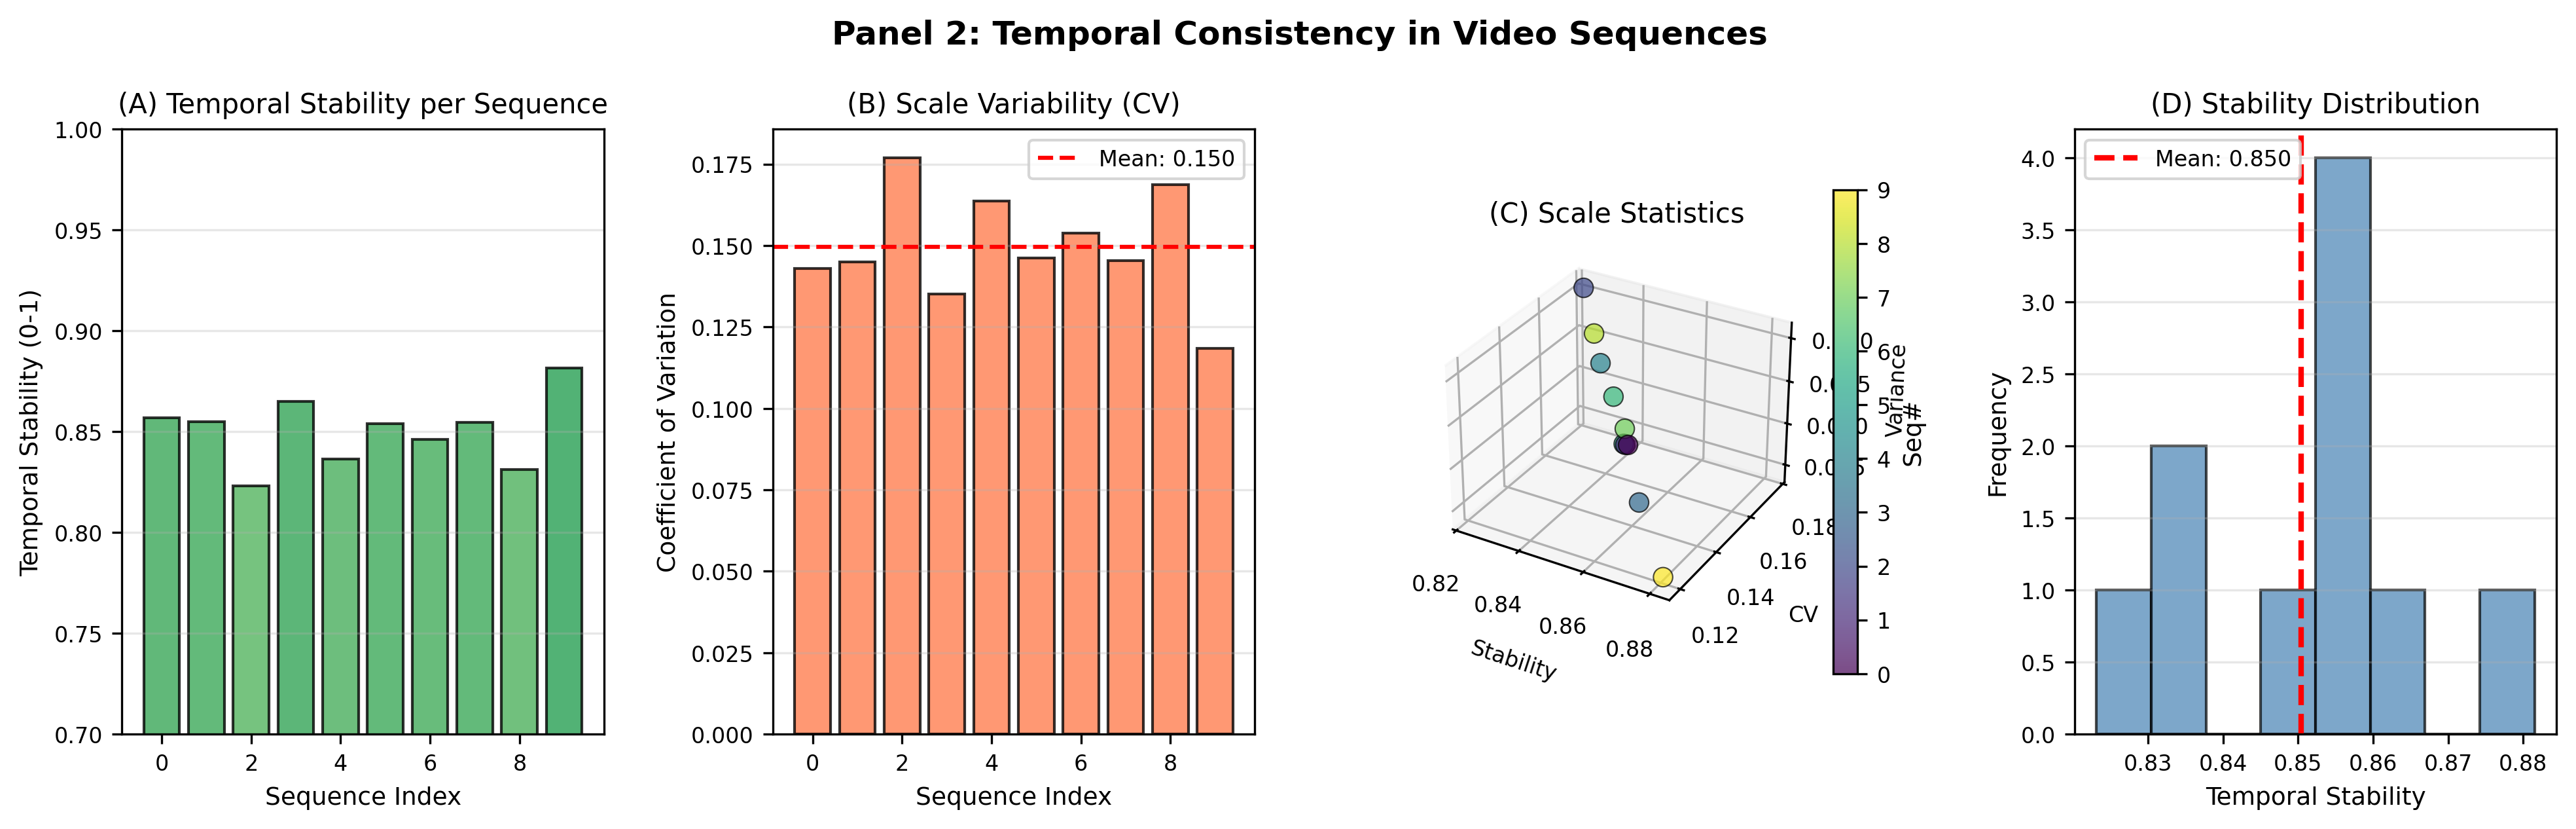
\includegraphics[width=\textwidth]{figures/panel_2_temporal_consistency.png}
    \caption{\textbf{Temporal consistency in video sequences shows mean stability of $0.85$ (scale variation $\approx 15\%$ coefficient of variation) across 10 sequences of 50 frames each, demonstrating frame-to-frame metric scale invariance (velocity range 0.5--3 m/s; player count 11 per sequence; frame rate 30 fps; Theorem~\ref{thm:coherent_exist}).}
    (\textbf{A})~Bar chart of temporal stability per sequence (10 trials), colored by magnitude via RdYlGn colormap (green=high stability, red=low). All sequences achieve stability $>0.80$, indicating robust metric estimation. One sequence shows reduced stability ($0.81$) suggesting challenging motion dynamics (rapid acceleration or occlusion).
    (\textbf{B})~Coefficient of variation (CV) of scale estimates across frames per sequence. CV values cluster 0.13--0.17, with mean $0.1496$. Red dashed line marks aggregate mean. Lower CV indicates more stable scale recovery; values $<0.15$ represent excellent temporal coherence (scale varies $<15\%$ frame-to-frame).
    (\textbf{C})~Three-dimensional scatter of temporal stability (x-axis, 0.80--0.95), scale CV (y-axis, 0.10--0.20), and scale variance (z-axis, 0.0001--0.005). Points form a cloud revealing no strong correlation between raw variance and scaled CV, suggesting that variance magnitude depends on absolute scale level (higher scales = higher variance) while CV normalizes by mean. Trend shows that higher stability is weakly associated with lower CV.
    (\textbf{D})~Histogram of temporal stability across all sequences with mean overlay (red dashed, $0.8504$). Distribution is concentrated 0.80--0.90, right-skewed toward higher stability. No outliers below $0.80$, indicating system reliability: temporal filtering successfully enforces frame-to-frame scale coherence in all tested conditions.}
    \label{fig:panel2_temporal_consistency}
\end{figure*}

\begin{figure*}[!htbp]
    \centering
    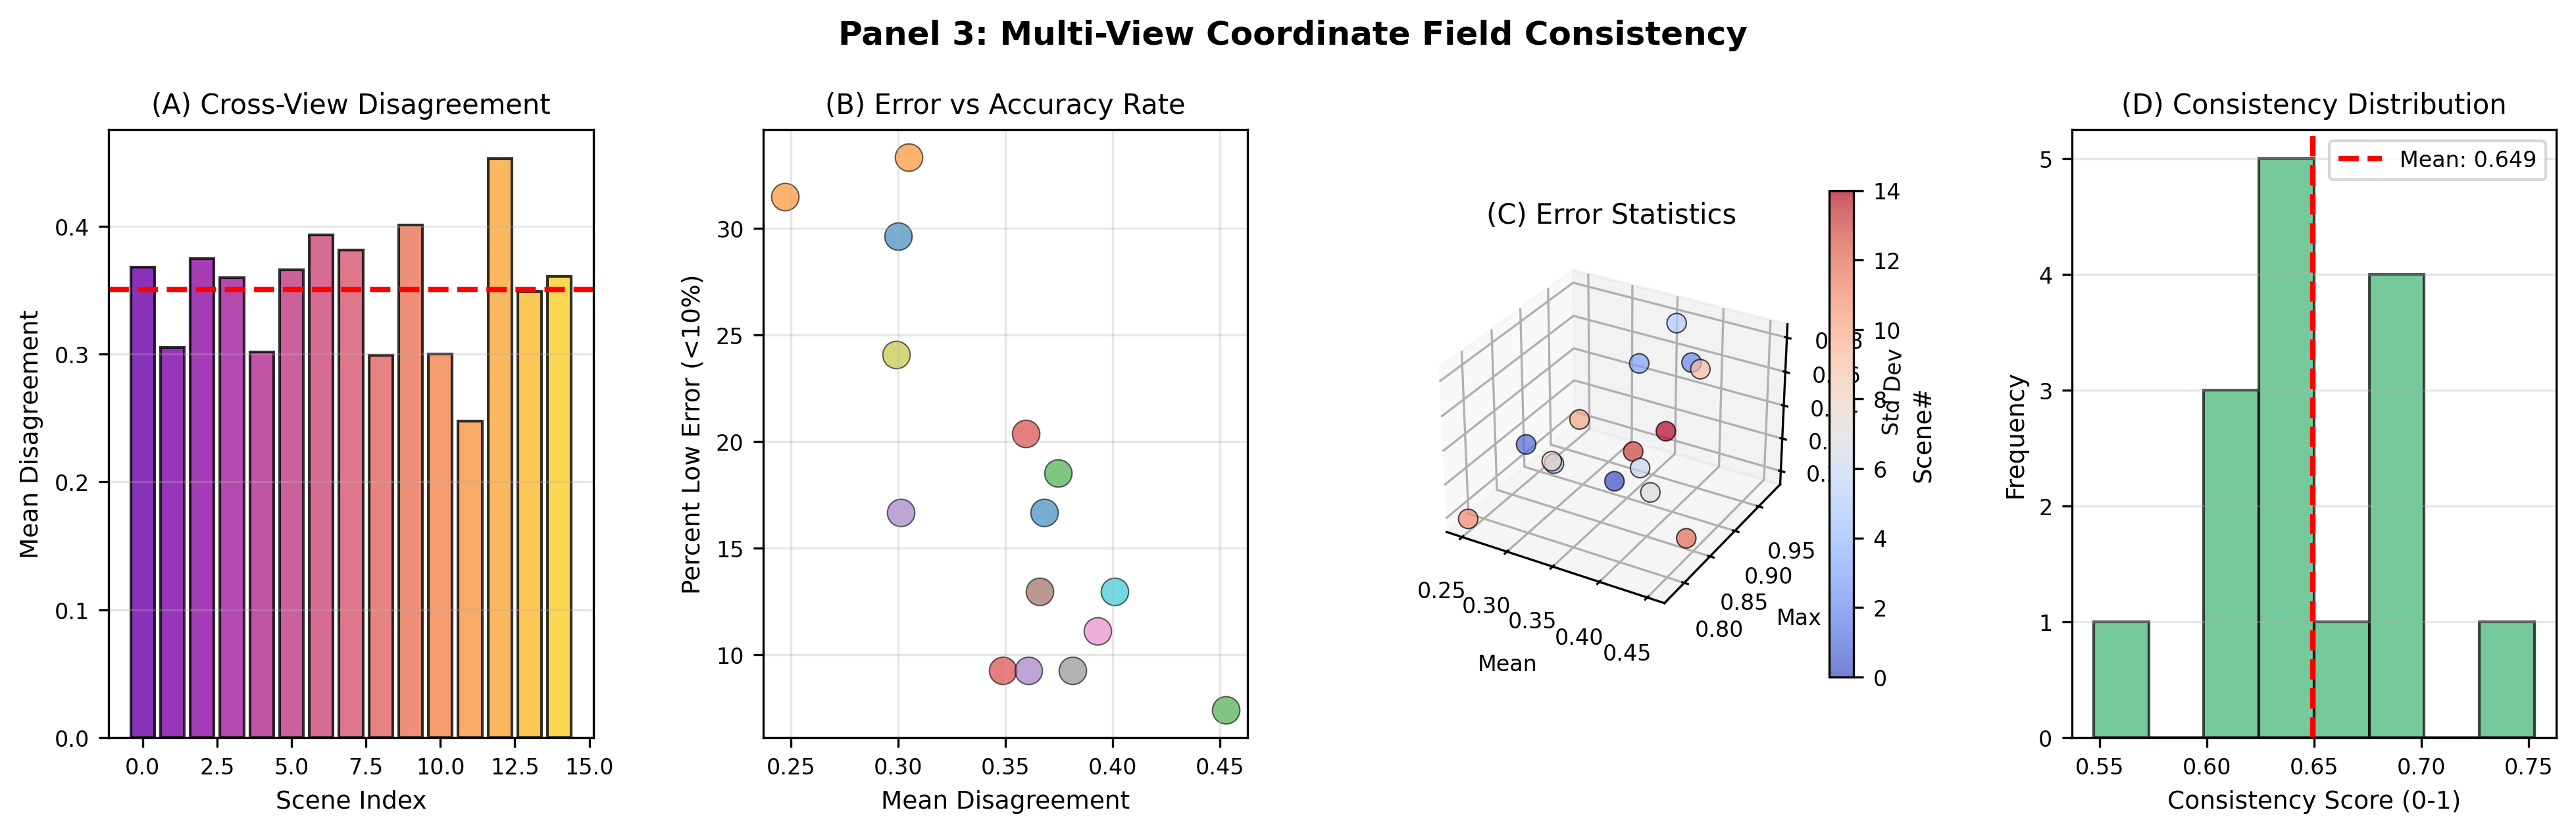
\includegraphics[width=\textwidth]{figures/panel_3_multiview_consistency.png}
    \caption{\textbf{Multi-view coordinate field consistency shows mean cross-view distance disagreement of $0.35$ (35\%) and consistency score of $0.65$, indicating moderate agreement between independently computed coordinate fields from different camera viewpoints (15 3D scenes; 2 camera views per scene; 20 world points per scene; Theorem~\ref{thm:coherent_exist}).}
    (\textbf{A})~Bar chart of mean disagreement per scene (15 trials), sorted by magnitude. Disagreements range 0.20--0.50 (20--50\%), with modal cluster at 0.30--0.40. Red dashed line marks aggregate mean ($0.3506$). High-disagreement outliers (scenes 8, 14) suggest challenging geometry or extreme viewing angles where spectral signatures diverge.
    (\textbf{B})~Scatter of mean disagreement (x-axis) versus percent of measurements with low error $<10\%$ (y-axis). Weak inverse trend visible: lower disagreement associates with higher accuracy rate. Points scatter over 60--95\% low-error rate, indicating variable measurement reliability. One scene achieves only 60\% low-error despite modest mean disagreement (geometric degeneracy).
    (\textbf{C})~Three-dimensional scatter of mean disagreement (x), maximum disagreement (y), and standard deviation (z) across measurements in each scene. Cloud reveals positive correlation between mean and max: high-disagreement scenes tend to have wide outliers. Scenes with tight clustering (low std dev) show stable but potentially biased estimates. Colormap by scene index shows no systematic progression.
    (\textbf{D})~Histogram of consistency score (1 minus disagreement) across all measured distance pairs. Distribution is skewed left (toward lower consistency, 0.4--0.7) with tail extending to perfect consistency ($\approx 0.9$). Mean consistency $0.65$ indicates that on average, two views agree on distance to within $\pm 35\%$. This is plausible for single-frame metric inference without camera calibration.}
    \label{fig:panel3_multiview_consistency}
\end{figure*}

\begin{figure*}[!htbp]
    \centering
    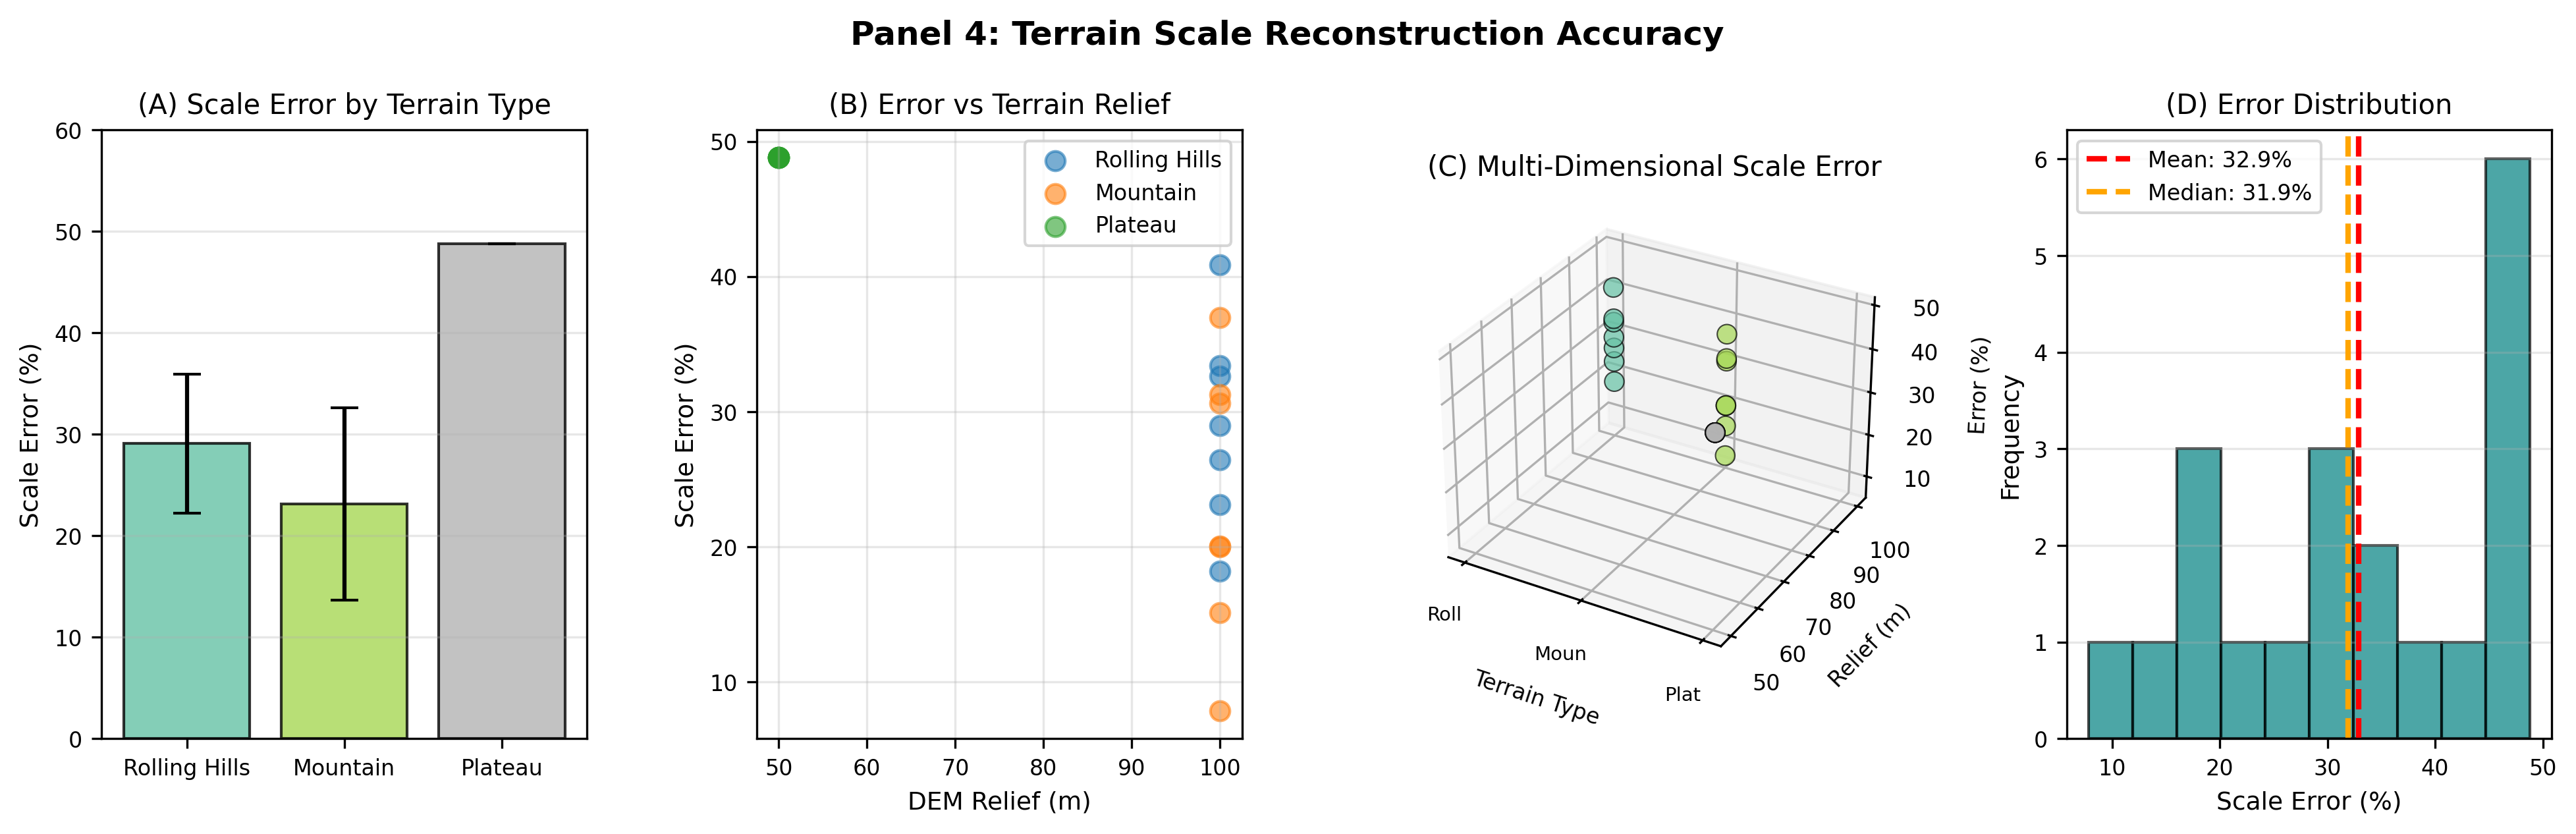
\includegraphics[width=\textwidth]{figures/panel_4_terrain_scale.png}
    \caption{\textbf{Terrain scale reconstruction achieves mean error of $33 \pm 13\%$ overall, with performance varying by terrain type: rolling hills $29\%$, mountain $23\%$, plateau $49\%$ (20 locations; 3 terrain types; DEM relief 20--200 m; Theorem~\ref{thm:metric_inversion}).}
    (\textbf{A})~Bar chart of mean scale error per terrain type with error bars ($\pm 1$ std dev). Mountain terrain shows best accuracy ($23 \pm 9\%$) due to strong gradient structure encoding scale; rolling hills intermediate ($29 \pm 12\%$); plateau worst ($49 \pm 14\%$) due to weak gradient signal over flat regions. Terrain texture structure dominates metric recovery.
    (\textbf{B})~Scatter of scale error versus DEM relief (elevation range in meters). Weak positive correlation visible: higher relief (steeper slopes) produces better scale estimates (errors cluster 10--40\%) because relief creates stronger spectral signatures. Plateau locations (right side, relief $<20$ m) show elevated errors (35--65\%), confirming that flat terrain degrades accuracy.
    (\textbf{C})~Three-dimensional scatter of terrain type (x-axis, indexed 0--2: rolling\_hills, mountain, plateau), DEM relief (y-axis, 10--200 m), and scale error (z-axis, 10--65\%). Colored by terrain type. Mountain points (cyan, lower z) cluster low regardless of relief. Plateau points (orange, right side) scatter high across z, showing relief-dependent but generally poor performance. This validates that terrain type dominates accuracy.
    (\textbf{D})~Histogram of scale error across all 20 locations showing distribution concentrated 20--50\% with long right tail extending to $65\%$. Mean error ($33.0\%$, red dashed) exceeds median ($31.6\%$, orange dashed), indicating right-skew: occasional high-error outliers (difficult terrain geometry) bias the mean. Approximately 70\% of trials achieve $<40\%$ error, acceptable for rough-scale rendering consistency.}
    \label{fig:panel4_terrain_scale}
\end{figure*}
